%; whizzy paragraph -pdf xpdf -latex ./whizzypdfptex.sh
%; whizzy-paragraph "^\\\\begin{frame}\\|\\\\emtext"
% latex beamer presentation.
% platex, latex-beamer $B$G%3%s%Q%$%k$9$k$3$H$rA[Dj!#(B 

%     Tokyo Debian Meeting resources
%     Copyright (C) 2012 Junichi Uekawa
%     Copyright (C) 2011 Nobuhiro Iwamatsu

%     This program is free software; you can redistribute it and/or modify
%     it under the terms of the GNU General Public License as published by
%     the Free Software Foundation; either version 2 of the License, or
%     (at your option) any later version.

%     This program is distributed in the hope that it will be useful,
%     but WITHOUT ANY WARRANTY; without even the implied warreanty of
%     MERCHANTABILITY or FITNESS FOR A PARTICULAR PURPOSE.  See the
%     GNU General Public License for more details.

%     You should have received a copy of the GNU General Public License
%     along with this program; if not, write to the Free Software
%     Foundation, Inc., 51 Franklin St, Fifth Floor, Boston, MA  02110-1301 USA

\documentclass[cjk,dvipdfm,12pt]{beamer}
\usetheme{Tokyo}
\usepackage{monthlypresentation}

%  preview (shell-command (concat "evince " (replace-regexp-in-string "tex$" "pdf"(buffer-file-name)) "&")) 
%  presentation (shell-command (concat "xpdf -fullscreen " (replace-regexp-in-string "tex$" "pdf"(buffer-file-name)) "&"))
%  presentation (shell-command (concat "evince " (replace-regexp-in-string "tex$" "pdf"(buffer-file-name)) "&"))
%  presentation (shell-command (concat "evince " (replace-regexp-in-string "tex$" "pdf"(buffer-file-name)) "&"))

%http://www.naney.org/diki/dk/hyperref.html
%$BF|K\8l(BEUC$B7O4D6-$N;~(B
\AtBeginDvi{\special{pdf:tounicode EUC-UCS2}}
%$B%7%U%H(BJIS$B7O4D6-$N;~(B
%\AtBeginDvi{\special{pdf:tounicode 90ms-RKSJ-UCS2}}

\title{$BEl5~%(%j%"(BDebian$BJY6/2q(B}
\subtitle{$BBh(B86$B2s(B 2012$BG/(B3$B7nEY(B}
\author{$B4d>>(B $B?.MN(B\\iwamatsu@debian.org\\Twitter: @iwamatsu}
\date{2012$BG/(B3$B7n(B17$BF|(B}
\logo{
\includegraphics[width=8cm]{image200607/openlogo-light.eps}}

\begin{document}

\frame{\titlepage{}}

\section{Agenda}

\begin{frame}{Agenda}
\begin{itemize}
\item $B:G6a$"$C$?(BDebian$B4XO"$N%$%Y%s%HJs9p(B
	\begin{itemize}
        \item $BBh(B85$B2s(B $BEl5~%(%j%"(BDebian$BJY6/2q(B
        \item $BBh(B0$B2s(B $BJ!2,(BDebian$BJY6/2q(B
	\end{itemize}
\item Debian $BJY6/2q(B -$B%f!<%6%5%$%I(B- Apache2 HTTP $B%5!<%P$+$i;O$a$k(BDebian
\item $B:#8e$N%$%Y%s%H(B
\end{itemize}
\end{frame}


\emtext{$B<+8J>R2p(B}

\begin{frame}{$B<+8J>R2p(B}
\begin{itemize}
\item $B4d>>(B $B?.MN(B $B!J$$$o$^$D(B $B$N$V$R$m!K(B / @iwamatsu
\item Debian Project Official Developer
\item Bluetooth, OpenCV, mozc, libpng $B$N%a%s%F%J(B
\item $BIaCJ$O(B Linux $B%+!<%M%k!"%V!<%H%m!<%@$J$I$r3+H/(B
\item $B!V(BGit$B$K$h$k%P!<%8%g%s4IM}!W$H$$$&K\$r=q$$$?$N$GGc$C$F$/$@$5$$(B
\end{itemize}
\end{frame}

\emtext{$BK\F|$N;qNA(B}
\begin{frame}{$BK\F|$N;qNA(B}

\begin{itemize}
\item $B%;%_%J!<%W%l%<%s%F!<%7%g%s(B\\
\url{http://tokyodebian.alioth.debian.org/2012-03.html}
\item $B%;%_%J!<%l%8%e%a(B
\url{http://tokyodebian.alioth.debian.org/2012-03.html}
\end{itemize}

$BA4It%a%b$r<h$kI,MW$O$"$j$^$;$s!#I,MW$J;v$@$1%a%b$r<h$j$^$7$g$&!#(B

\end{frame}

\emtext{$B%$%Y%s%HJs9p(B}

\begin{frame}{$BBh(B85$B2sEl5~%(%j%"(BDebian$BJY6/2q(B}
\begin{itemize}
\item Debian $B3+H/<T$N0Y$N(B KDE $B3+H/4D6-$K$D$$$F(B
\item $B7n4)(BDebhelper $BBh(B4$B2s(B
\item cmake $B$r;H$C$F$_$?(B
\end{itemize}
\end{frame}

\begin{frame}{$BBh(B0$B2sJ!2,(BDebian$BJY6/2q(B}

\begin{itemize}
\item $B$J$<$+J!2,$K9T$C$?$N$G!"JY6/2q$r$7$?!#(B
\item DKMS $B$N;EAH$_$H(B Debian $B$NBP1~>u67(B
\item Debian$B%5!<%PNL;:9)>l(B - $BL58B%]%A%]%A(B on Debian
\end{itemize}

\end{frame}

\emtext{Apache2 /HTTP $B%5!<%P$+$i;O$a$k(B Debian}

\section{Apache2 /HTTD $B%5!<%P$+$i;O$a$k(B Debian}

% [plain]
% [containsverbatim]
\begin{frame}[plain]

\begin{itemize}
\item $BIaCJ$O$A$g$C$H3+H/<T4s$j$JOC$r$7$F$$$k(B Debian $BJY6/2q(B..\pause
\item Debian $BJY6/2q$O62$m$7$$=j!*(B\pause $B$G$O$J$$!#(B\pause
\item $B:#2s$O(B OSC $B=PD%4k2h$H$7$F!"%f!<%6!<;kE@$NJY6/2q$r3+:E!#(B\pause
\item $B%f!<%6%5%$%I!)%f!<%68~$1$N(BDebian$BJY6/2q!#(B\pause
\item $B%f!<%6$N@8$N0U8+$r<h$jF~$l!"(BDebian$B!"(BUpsteam$B$KH?1G!J$G$-$k$+$b!K!#(B
\item $BH?1~$,NI$1$l$P<!2s$b$"$k$+$b$7$l$^$;$s!#(B
\end{itemize}

\end{frame}

\begin{frame}
\begin{center}
\Huge{$B$O$8$a$K(B}
\end{center}
\end{frame}


\begin{frame}{$B$O$8$a$K(B}

\begin{itemize}
\item $B1=$K$h$k$H!"(BDebian $B$O(B $B@$3&!J%h!<%m%C%Q!K$G(BHTTP$B%5!<%P$H$7$F0lHV:NMQ$5$l$F$$$k(B Linux $B%G%#%9%H%j%S%e!<%7%g%s$i$7$$!#(B\footnote{\url{http://w3techs.com/blog/entry/debian_is_now_the_most_popular_linux_distribution_on_web_servers}}\pause
\item $BF|K\$G$O(B HTTP $B%5!<%P$H$7$F$"$^$jMxMQ$5$l$F$$$k$h$&$K8+$($^$;$s$,!#(B

\end{itemize}

\end{frame}

\begin{frame}{$B$O$8$a$K(B}

\begin{itemize}
\item $BMxMQ$5$l$F$$$kM}M3$O(B HTTP $B%5!<%P%Q%C%1!<%8$N<oN`$,B?$/$"$k;v$,M}M3$N0l$D$@$H$+!#(B
\item Apache HTTPD$B!"(BNginx$B!"(BLighttpd$B!"(Betc..
\end{itemize}

\end{frame}

\begin{frame}{$B$O$8$a$K(B}

\begin{itemize}
\item $B<B:]$KMxMQ$7$F$$$k?M!J>&6HMxMQ!K$KJ9$/$HM}M3$O$3$l$@$1$G$O$J$$$h$&$@!#(B\pause
\item Debian$B$N%Q%C%1!<%8%s%0%7%9%F%`(B\pause
\item APT\pause
\item Apahce $B%b%8%e!<%k%Q%C%1!<%8$NB?$5(B \pause
\item Web$B%"%W%j%1!<%7%g%s$G:NMQ$5$l$k(B P$B8@8l!J(BPerl, Python, PHP$B!KEy$N%5%]!<%H(B\pause
\item {\color{red}$B@_Dj%U%!%$%k$N=@Fp@-(B}
\end{itemize}

\end{frame}


\begin{frame}{$B@_Dj%U%!%$%k$N=@Fp@-(B}

\begin{itemize}
\item Debian $B$C$F$d$d$3$7$$%$%a!<%8(B ($B$i$7$$(B)\pause
\item Red Hat $B7O(B $B$H0c$$!"(BDebian $BFCM-$N@_Dj%U%!%$%k$N9=@.(B \pause
\item $B$7$+$7$J$<FCM-$N9=@.$K$J$C$F$$$k$N$+!)(B \pause
\item $BM}2r$9$k$H!"B>$N%G%#%9%H%j%S%e!<%7%g%s$H$N%a%j%C%H!"%G%a%j%C%H$,8+$($F$/$k$O$:!#(B
\end{itemize}

\end{frame}

\begin{frame}{$B$O$8$a$K(B}

$B$H$$$&$o$1$G:#2s$O!"(BDebian $B$N(B Apache2 / HTTP $B%5!<%P(B ($B0J2<!"(BApache2 $B!K(B $B$K$D$$$FJY6/$7$^$7$g$&!#(B

\end{frame}

\begin{frame}
\begin{center}
\Huge{Debian $B$N(B Apache2\\$B%P!<%8%g%s(B}
\end{center}
\end{frame}

\begin{frame}{Debian $B$N(B Apache2 $B%P!<%8%g%s(B}

\begin{center}
\begin{tabular}{|l|l|}
\hline 
$B%G%#%9%H%j%S%e!<%7%g%s(B & $B%P!<%8%g%s(B \\
\hline \hline
stable & 2.2.16-6+squeeze6 \\
\hline
testing & 2.2.22-1 \\
\hline
unstable & 2.2.22-1 \\
\hline
experimental &  - \\
\hline
Upstream & 2.4.1 \\
\hline
\end{tabular}
\end{center}

\pause

\begin{itemize}
\item Upstream $B$HHf$Y$k$H>/$78E$$$,!"5!G=E*$K$OLdBj$J$$!#(B
\item $B$b$A$m$s%;%-%e%j%F%#%"%C%W%G!<%H$K$bBP1~!#(B
\item RHEL$B!"(BCentOS$B!J(B\texttt{$B%P!<%8%g%s(B 2.2.15-15}$B!K$HHf$Y$F$bFC$K%P!<%8%g%s$,8E$$$H$$$&$o$1$G$b$J$$!#(B
\end{itemize}

\end{frame}

\begin{frame}[plain]

\begin{center}
\Huge{Debian $B$N%Q%C%1!<%89=@.$H%Q%C%1!<%8$N%$%s%9%H!<%k(B}
\end{center}

\end{frame}

\begin{frame}{$B%Q%C%1!<%89=@.(B}

\begin{center}
\begin{tabular}{|l|l|}
\hline 
$B%Q%C%1!<%8L>(B & $B%Q%C%1!<%8$N@bL@(B\\
\hline \hline 
apache2 & Apache HTTP $B%5!<%P%a%?%Q%C%1!<%8(B \\
\hline
apache2-mpm-worker & $B%9%l%C%I%b%G%k(B HTTP $B%5!<%P(B\\
\hline 
apache2-mpm-prefork & $BHs%9%l%C%I%b%G%k(B HTTP $B%5!<%P(B\\ 
\hline
apache2-mpm-event & $B%$%Y%s%H%I%j%V%s%b%G%k(B HTTP $B%5!<%P(B\\ 
\hline 
apache2-mpm-itk & $B%^%k%A%f!<%64D6-(B HTTP $B%5!<%P(B\\
\hline
apache2.2-common & Apache HTTP $B%5!<%P(B $B6&DL%U%!%$%k(B \\
\hline
apache2.2-bin & Apache HTTP $B%5!<%P(B $B6&DL%P%$%J%j(B\\ 
\hline
apache2-utils & $B%&%'%V%5!<%PMQ%f!<%F%#%j%F%#(B \\
\hline
apache2-suexec & mod-suexec $BMQ(B $B4pK\(B suexec \\
\hline
apache2-suexec-custom & mod-suexec $BMQ(B $B@_Dj2DG=(B suexec \\
\hline
apache2-doc & Apache HTTP $B%5!<%P%I%-%e%a%s%H(B \\
\hline
\end{tabular}
\end{center}

\end{frame}


\begin{frame}{$B%Q%C%1!<%89=@.(B}

\begin{center}
\begin{tabular}{|l|p{16em}|}
\hline 
$B%Q%C%1!<%8L>(B & $B%Q%C%1!<%8$N@bL@(B\\
\hline \hline
apache2-dbg & Apache HTTP $B%5!<%P(B $B%G%P%C%0%7%s%\%k%U%!%$%k(B \\
\hline
apache2-prefork-dev & $BHs%9%l%C%I%b%G%k(B HTTP $B%5!<%P(B $B3+H/MQ%U%!%$%k(B\\
\hline
apache2-threaded-dev & $B%^%k%A%9%l%C%I%b%G%k(B HTTP $B%5!<%P(B $B3+H/MQ%U%!%$%k(B \\
\hline
\end{tabular}
\end{center}

\end{frame}

\begin{frame}{$B%Q%C%1!<%89=@.(B}

\begin{itemize}
\item HTTP $B%5!<%P$N=hM}%b%G%k$4$H$K%Q%C%1!<%8(B
$B!J(Bapache2-mpm-worker$B!"(Bapache2-mpm-prefork$B!"(Bapache2-mpm-event$B!"(Bapache2-mpm-itk$B!K(B
$B$,J,N%$5$l$F$$$k!#(B
\item $BMQES$K9g$o$;$?%Q%C%1!<%8$r%$%s%9%H!<%k$G$-$k!#(B
\item Red Hat$B7O$O0l$D$N%Q%C%1!<%8$KE;$^$C$F$$$F!"=hM}%b%G%kKh$K%5%U%#%C%/%9$r$D$1$F$$$k!JNc!'(Bhttpd.worker$B!K!#(B
\end{itemize}

\end{frame}

\begin{frame}

\begin{center}
\Huge{$B%Q%C%1!<%80MB84X78(B}
\end{center}

\end{frame}

\begin{frame}{$B%Q%C%1!<%80MB84X78(B}

\begin{center}
  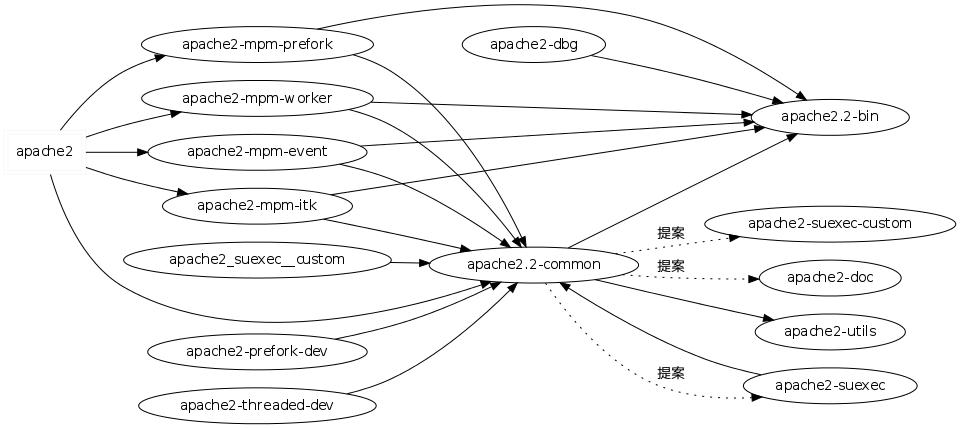
\includegraphics[width=1.0\hsize]{image201203/apache2-pkg.png}
\end{center}


\end{frame}

\begin{frame}{$B%Q%C%1!<%80MB84X78(B}

\begin{itemize}
\item $B0MB84X78$,J#;($J$N$G%f!<%6$OIT0B$K$J$k$+$b$7$l$J$$!#(B
\item Debian$B$G$O6/NO$J%Q%C%1!<%84IM}%D!<%k(B APT $B$K$h$C$F5$$K$9$k;v$J$/%$%s%9%H!<%k$G$-$k!#(B
\end{itemize}

\end{frame}

\begin{frame}

\begin{center}
\Huge{$B%$%s%9%H!<%k(B}
\end{center}

\end{frame}

\begin{frame}[containsverbatim]{$B%$%s%9%H!<%k(B}

\begin{itemize}
\item Debian$B$G(B $B%Q%C%1!<%8$r%$%s%9%H!<%k$9$k>l9g!"(B \texttt{apt-get install}$B%3%^%s%I$r;H$&!#(B
\item apache2 $B$H$$$&%a%?%Q%C%1!<%8$r;H$C$F%$%s%9%H!<%k$9$k$3$H$,B?$$!#(B

\begin{commandline}
$ sudo apt-get update
$ sudo apt-get install apache2
\end{commandline}

\item $B%G%U%)%k%H$O(B apache2-mpm-worker$B!J%9%l%C%I%b%G%k(B HTTP $B%5!<%P!K$,%$%s%9%H!<%k$5$l$k!#(B
\item $BB>$N(B HTTP $B%5!<%P%Q%C%1!<%8$r%$%s%9%H!<%k$7$?$$>l9g$O!"3F!9$N%Q%C%1!<%8$r(B
$B;XDj$7$F%$%s%9%H!<%k$9$kI,MW$,$"$k!#(B
\end{itemize}

\end{frame}

\begin{frame}{$B%$%s%9%H!<%k(B}

\begin{itemize}
\item CentOS$B$J$I$G$O!"!V(Bhttpd$B!W(B $B%Q%C%1!<%8$H$7$FDs6!$5$l$F$$$k$N$G%Q%C%1!<%8L>$,0[$J$k!#(B
\item $BIaCJ$OB>$N%G%#%9%H%j%S%e!<%7%g%s$r;H$C$F$$$k?M$OCm0U$9$k$3$H!#(B
\end{itemize}
\end{frame}

\begin{frame}

\begin{center}
\Huge{Apache HTTP $B%5!<%P$N5/F0$HDd;_(B}
\end{center}

\end{frame}

\begin{frame}{Apache HTTP $B%5!<%P$N5/F0$HDd;_(B}

\begin{itemize}
\item Debian $B$O!V%$%s%9%H!<%k$7$?$b$N$O;H$&!W$H$$$&%]%j%7!<!#(B\pause
\item $B%Q%C%1!<%8%$%s%9%H!<%k40N;$N;~E@$G4{$K(B Apache HTTP $B%5!<%P$O5/F0$7$F$$$k!#(B\pause
\item $BDd;_$7$?$$>l9g(B:\\
\texttt{sudo /etc/init.d/apache2 stop} \pause
\item $B5/F0$7$?$$>l9g(B:\\
\texttt{sudo /etc/init.d/apache2 start} \pause
\item $B:F5/F0$7$?$$>l9g(B:\\
\texttt{sudo /etc/init.d/apache2 restart}
\end{itemize}

\end{frame}

\begin{frame}[containsverbatim]{Apache HTTP $B%5!<%P$N5/F0$HDd;_(B}

\begin{commandline}
$ ps ax | grep apache2
10034 ?      Ss   0:05 /usr/sbin/apache2 -k start
13008 ?      S    0:00 /usr/sbin/apache2 -k start
....
$ sudo /etc/init.d/apache2 stop
$ ps ax | grep apache2
16833 pts/1  S+   0:00 grep apache2 
$ sudo /etc/init.d/apache2 start
$ ps ax | grep apache2
10048 ?      Ss   0:05 /usr/sbin/apache2 -k start
13024 ?      S    0:00 /usr/sbin/apache2 -k start
....
\end{commandline}
%$

\end{frame}

\begin{frame}{Apache HTTP $B%5!<%P$N5/F0$HDd;_(B}

\begin{itemize}
\item $B%G%U%)%k%H$N>uBV$G$O!"%^%7%s$rN)$A>e$2;~$K(B HTTP $B%5!<%P$,5/F0$9$k$h$&$K$J$C$F$$$k!#(B\pause
\item $B5/F0$7$J$$$h$&$K$9$k$K$O!"%i%s%l%Y%kKh$KF0:n$9$k%5!<%P!J%5!<%S%9!KJQ99$9$kI,MW$,$"$k!#(B\pause
\item $B%5!<%S%9$N5/F0@_Dj(B $\rightarrow$ \texttt{update-rc.d} $B%3%^%s%I$r;H$&!#(B
\end{itemize}

\end{frame}

\begin{frame}[containsverbatim]{Apache HTTP $B%5!<%P$N5/F0$HDd;_(B}

\begin{itemize}
\item $BA4$F$N%i%s%l%Y%k$G(B Apache2 $B$r5/F0$5$;$J$$$h$&$K@_Dj(B:\\
\texttt{sudo update-rc.d -f apache2 remove}

\item $B%$%s%9%H!<%kD>8e$N%G%U%)%k%H$N>uBV$KLa$7$?$$>l9g(B:\\
\texttt{sudo update-rc.d -f apache2 default}
\end{itemize}

\end{frame}

\begin{frame}{Apache HTTP $B%5!<%P$N5/F0$HDd;_(B}

\begin{itemize}
\item Red Hat$B7O$@$H(B \texttt{chkconfig} $B$r;H$&!#(B\pause
\item Debian $B$K$O$J$$$s$G$7$g!)(B \pause $B$b$A$m$s(BDebian$B$G$bDs6!$5$l$F$$$k!#(B\pause
\item \texttt{chkconfig} $B$O(B RedHat$B7O$N%5!<%S%94IM}%D!<%k$J$N$G(B....$B!#(B\pause
\item $B%$%s%?!<%U%'%$%9$,;w$F$$$k(B \texttt{sysv-rc-conf}$B$,$"$k$N$G$3$A$i$r;H$&!#(B
\end{itemize}

\end{frame}


\begin{frame}[containsverbatim]{Apache HTTP $B%5!<%P$N5/F0$HDd;_(B}

\begin{itemize}
\item $B8=:_$N>uBV$r=PNO(B:\\
\texttt{sudo sysv-rc-conf --list}

\item $B%i%s%l%Y%k(B2$B$N(Bapache2$B$rL58z$K$9$k(B:\\
\texttt{sudo sysv-rc-conf --level 2 apache2 off}

\item $B%i%s%l%Y%k(B2$B$N(Bapache2$B$rM-8z$K$9$k(B:\\
\texttt{sudo sysv-rc-conf --level 2 apache2 on}

\end{itemize}

\end{frame}


\begin{frame}[containsverbatim]{Apache HTTP $B%5!<%P$N5/F0$HDd;_(B}

\begin{commandline}
$ sudo apt-get install sysv-rc-conf 
$ sudo sysv-rc-conf --list
apache2      0:off1:off2:on3:on4:on5:on6:off
bootlogd     S:on
$B!JCfN,!K(B
$ sudo sysv-rc-conf --level 2 apache2 off 
$ sudo sysv-rc-conf --list | head -1 
apache2      0:off1:off2:off3:off4:off5:off6:off
$ sudo sysv-rc-conf --level 2 apache2 on
$ sudo sysv-rc-conf --list | head -1
apache2      0:off1:off2:on3:off4:off5:off6:off
\end{commandline}
%$

\end{frame}

\begin{frame}
\begin{center}
\Huge{Apache2 $B$N@_Dj%U%!%$%k(B}
\end{center}
\end{frame}

\begin{frame}{Apache2 $B$N@_Dj%U%!%$%k(B}

\begin{itemize}
\item Red Hat $B7O$N>l9g(B
\begin{itemize}
\item $B<g$J@_Dj$O(B \texttt{/etc/httpd/conf/httpd.conf}$B$G9T$&(B
\item include $B$5$l$k%U%!%$%k$O(B \texttt{/etc/httpd/conf.d/}$B%G%#%l%/%H%j$K3JG<$9$k!#(B
\end{itemize}
\end{itemize}

\end{frame}

\begin{frame}{Apache2 $B$N@_Dj%U%!%$%k(B}

Debian $B$N>l9g(B


\begin{center}
\begin{tabular}{|l|p{12em}|}
\hline 
$B@_Dj%U%!%$%k(B & $BFbMF(B\\
\hline \hline
/etc/apache2/apache2.conf & $B4pK\@_Dj(B\\
\hline
/etc/apache2/httpd.conf & $B%*!<%P!<%i%$%I$9$k@_Dj(B\\
\hline
/etc/apache2/conf.d/ & Include$B$9$k%U%!%$%k$r3JG<(B\\
\hline
/etc/apache2/ports.conf & $B%]!<%H$N@_Dj(B\\
\hline
/etc/apache2/envvars & $B4D6-JQ?t$N@_Dj(B\\
\hline
/etc/apache2/mods-available/ & $BMxMQ2DG=$J%b%8%e!<%k@_Dj(B\\
\hline
/etc/apache2/mods-enabled/ & $BMxMQCf$N%b%8%e!<%k@_Dj(B\\
\hline
/etc/apache2/sites-available/ & $BMxMQ2DG=$J%5%$%H@_Dj(B\\
\hline
/etc/apache2/sites-enabled/ & $BMxMQCf$N%5%$%H@_Dj(B\\
\hline
/var/www & $B%I%-%e%a%s%H%k!<%H(B\\
\hline
/usr/lib/cgi-bin & cgi-bin\\
\hline
/var/log/apache2 & Apache2 $B%m%0(B\\
\hline
\end{tabular}
\end{center}

\end{frame}



\begin{frame}[containsverbatim]{Apache2 $B$N@_Dj(B}
\begin{center}

\begin{center}
  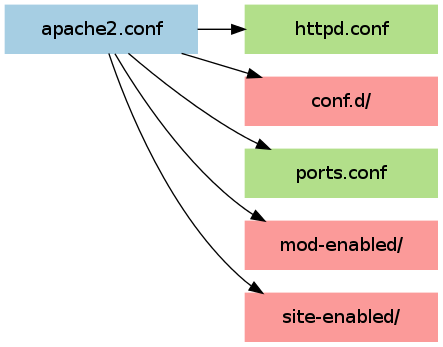
\includegraphics[width=0.9\hsize]{image201203/apache2-file.png}
\end{center}

\end{center}
\end{frame}

\begin{frame}[containsverbatim]{Apache2 $B$N@_Dj(B}

\begin{itemize}
\item \texttt{apache2.conf}$B$K$O0J2<$N9T$,$"$j!"(B\texttt{apache2.conf}
$B$+$i3F@_Dj$,FI$_9~$^$l$k$h$&$K$J$C$F$$$k!#(B

\begin{commandline}
$B!J>JN,!K(B
# Include module configuration:
Include /etc/apache2/mods-enabled/*.load
Include /etc/apache2/mods-enabled/*.conf

# Include all the user configurations:
Include /etc/apache2/httpd.conf

# Include ports listing
Include /etc/apache2/ports.conf
$B!JCfN,!K(B
# Include generic snippets of statements
Include /etc/apache2/conf.d/

# Include the virtual host configurations:
Include /etc/apache2/sites-enabled/
\end{commandline}

\end{itemize}

\end{frame}


\begin{frame}{Apache2 $B$N@_Dj(B}

\begin{itemize}
\item Apache2 $B$N@_Dj$rJQ99$9$k>l9g!"(B\texttt{apache2.conf}$B$rJQ99$7$J$$!#(B
\item \texttt{httpd.conf} $B$d(B \texttt{ports.conf}$B$rJQ99$9$k!#(B
\end{itemize}

\end{frame}


\begin{frame}
\begin{center}
\Huge{$B%5%$%H$N@_Dj(B}
\end{center}
\end{frame}


\begin{frame}[containsverbatim]{$B%5%$%H$r@_Dj$9$k(B}

\begin{itemize}
\item Debian $B$O(B\texttt{/etc/apache2/sites-available/default} $B$K(B apache2 $B$N%G%U%)%k%H$N%5%$%H@_Dj(B
$B$r3JG<$7$F$$$k!#(B
\item $B%5%$%H$r0l$D$@$19=C[$9$k>l9g$O$3$N%U%!%$%k$rJQ99$9$k!#(B
\item $BJQ99$7$?8e$O!"(Bapache2 $B$r:F5/F0$9$k!#(B
\item $B:F5/F0J}K!(B\\

\begin{commandline}
$ sudo /etc/init.d/apache2 restart
\end{commandline}
%$

\end{itemize}
\end{frame}


\begin{frame}[containsverbatim]{$B%5%$%H$N@_Dj(B}

\begin{itemize}
\item Debian $B$N(B Apache2 $B$GJ#?t$N%5%$%H$rN)$A>e$2$k>l9g!"(Bapache2.conf $B$OJT=8$7$J$$!#(B
\item $B%5%$%HJL$K@_Dj$r5-=R$7!"(B\texttt{/etc/apache2/sites-available/}$B%G%#%l%/%H%j$K3JG<$9$k!#(B
\item $B$=$N%5%$%H@_Dj$rM-8z$K$9$k%3%^%s%I!V(B\texttt{a2ensite}$B!W<B9T$7!"(BApache2 $B$r:F5/F0$9$k!#(B
\end{itemize}

\end{frame}

\begin{frame}[containsverbatim]{$B%5%$%H$N@_Dj(B}


%\begin{commandline}
%
%<VirtualHost *>
%    ServerAdmin admin-test@example.org
%    ServerName test.example.org
%    DocumentRoot /home/test/public_html/
%    <Directory />
%        Options FollowSymLinks ExecCGI Includes
%        AllowOverride None
%    </Directory>
%</VirtualHost>
%\end{commandline}

\begin{enumerate}
\item $B%5%$%H@_Dj$r5-=R$9$k!J(Btest $B$H$9$k(B)$B!#(B
\item $B%5%$%H@_Dj$r(B\texttt{/etc/apache2/sites-available/test}$B$K3JG<$9$k!#(B
\item \texttt{sudo a2ensite test}$B$r<B9T$9$k!#(B\\
$B<B9T$9$k$H(B\texttt{/etc/apache2/sites-enabled/}
$B$K%7%s%\%j%C%/%j%s%/$,D%$i$l@_Dj$,M-8z$K$J$k!#(B
\item Apache2 $B$r:F5/F0$9$k!#(B\\
$BM-8z$K$7$?$@$1$G$O!"2TF/$7$F$$$k(Bhttpd $B%5!<%P$K$O@_Dj$,H?1G$5$l$F$$$J$$$?$a!#(B
\end{enumerate}

\end{frame}

\begin{frame}[containsverbatim]{$B%5%$%H$N@_Dj(B}
\begin{commandline}
$ ls -F /etc/apache2/sites-enabled/
000-default@  default-ssl.old@
$ sudo a2ensite test
Enabling site test.
Run '/etc/init.d/apache2 reload' to activate new configuration!
$ ls -l /etc/apache2/sites-enabled/
000-default@  test@  default-ssl.old@
$ sudo /etc/init.d/apache2 restart
\end{commandline}

\end{frame}

\begin{frame}[containsverbatim]{$B%5%$%H$N@_Dj$rL58z$K$9$k(B}

\begin{itemize}
\item $B%5%$%H$N@_Dj$rL58z$K$9$k>l9g!"!V(B\texttt{a2dissite}$B%3%^%s%I!W$KL58z$K$7$?$$%5%$%H$N@_Dj%U%!%$%kL>$r;XDj$7$F<B9T$9$k!#(B
\item $B<B9T$9$k$H(B\texttt{/etc/apache2/sites-enabled/}$B$+$i%7%s%\%j%C%/%j%s%/$,:o=|$5$l$k!#(B
\item $B%5%$%H@_Dj$rL58z$K$7$?8e$O!"M-8z;~$HF1MM$K(B Apache2 $B$r:F5/F0$9$kI,MW$,$"$k!#(B
\end{itemize}

\begin{commandline}
$ sudo a2dissite test
Site test disabled.
Run '/etc/init.d/apache2 reload' to activate new configuration!
$ ls -l /etc/apache2/sites-enabled/ 
000-default@  default-ssl.old@
\end{commandline}
%$

\end{frame}

\begin{frame}[containsverbatim]{$B%5%$%H$N@_Dj$rL58z$K$9$k(B}

\begin{itemize}
\item Debian$B$G$O%5%$%H$N@_Dj$rJ,N%$7!"%5%$%HKh$K>uBV$r4IM}$9$k$3$H$,$G$-$k!#(B
\item $BB>$N%G%#%9%H%j%S%e!<%7%g%s$G$O(B \texttt{include} $BEy$r;H$C$F4IM}$G$-$k$,!"(B
$B%U%!%$%kFbMF$rJQ99$9$kI,MW$,$"$k$N$GHs>o$K<j4V!#(B
\item Debian $B$O%7%s%\%j%C%/%j%s%/$r;H$&$3$H$K$h$C$F(BApache2 $B$N@_Dj%U%!%$%k$r(B
$BJQ99$;$:$K%5%$%H@_Dj$NM-8z!&L58z$,$G$-$k!#(B
\end{itemize}

\end{frame}


\begin{frame}
\begin{center}
\Huge{$B%b%8%e!<%k$N@_Dj(B}
\end{center}
\end{frame}


\begin{frame}[containsverbatim]{$B%b%8%e!<%k$rM-8z(B/$BL58z$K$9$k(B}

\begin{itemize}
\item  Debian $B$N%b%8%e!<%k$K4X$9$k@_Dj$O%b%8%e!<%kKh$N@_Dj%U%!%$%k$H$7$F(B
\texttt{mods-available}$B%G%#%l%/%H%j$K3JG<$5$l$F$$$k!#(B
\item $B$=$l$i$N$&$A!"<B:]$KM-8z$J$b$N$,(B \texttt{mods-enabled} $B%G%#%l%/%H%j$K%7%s%\%j%C%/%j%s%/$,D%$i$l$k!#(B
\item $B%7%s%\%j%C%/%j%s%/$O<jF0$G9T$o$J$$!#(B
\item $B%b%8%e!<%k$rM-8z$K$9$k>l9g$K$O(B\texttt{a2enmod}$B%3%^%s%I$r;H$&!#(B
\item $BL58z$K$9$k>l9g$K$O(B\texttt{a2dismod}$B%3%^%s%I$r;H$&!#(B
\item $BM-8z!&L58z$K$7$?8e$O(B Apache2 $B$r:F5/F0$9$k!#(B
\end{itemize}

\end{frame}

\begin{frame}[containsverbatim]{$BNc(B: mod\_info $B$rM-8z$K$9$k(B}

\begin{commandline}
$ ls -l /etc/apache2/mods-enabled/ | grep info 
$B!J=PNO$J$7!K(B
$ sudo a2enmod info
Enabling module info.
Run '/etc/init.d/apache2 restart' to activate new configuration!
$ sudo /etc/init.d/apache2 restart
.....
$ sudo /usr/sbin/apache2ctl -D DUMP_MODULES 2>/dev/null | grep info 
  info_module (shared)
\end{commandline}
%$

\end{frame}

\begin{frame}[containsverbatim]{$BNc(B: mod\_info $B$rL58z$K$9$k(B}

\begin{commandline}
$ ls -l /etc/apache2/mods-enabled/ | grep info 
info.conf@
info.load@
$ sudo a2dismod info
Module info disabled.
Run '/etc/init.d/apache2 restart' to activate new configuration!
$ ls -l /etc/apache2/mods-enabled/ | grep info 
$ sudo '/etc/init.d/apache2 restart
.....
$ sudo /usr/sbin/apache2ctl -D DUMP_MODULES 2>/dev/null | grep info
$B!J=PNO$J$7!K(B
\end{commandline}
%$

\end{frame}


\begin{frame}{$B$=$NB>(B}

\begin{center}
\Huge{$B$=$NB>(B}
\end{center}

\end{frame}

\begin{frame}{libapache2-mod-php5 $B$H(B apache2-mpm-prefork}

\begin{itemize}
\item apache2-mpm-worker$B!J%9%l%C%I%b%G%k!K(B $B$G(B PHP5$B!J(Bmod-php5$B!K(B $B$O;H$($J$$!#(B
\item PHP5$B!J(Bmod-php5$B!K$N@)8B$G!"%9%l%C%I%;!<%U$G$O$J$$$?$a!#(B
\item apache2-mpm-prefork $B!JHs%9%l%C%I%b%G%k!K$r;H$&I,MW$,$"$k!#(B
\item libapache2-mod-php5 $B$r%$%s%9%H!<%k$9$k$H!"(Bapache2-mpm-worker $B$,:o=|$5$l!"(Bapache2-mpm-prefork $B$,%$%s%9%H!<%k$5$l$k!J?F@Z@_7W!K!#(B
\item PHP $B%f!<%6$NJ}$OCm0U$7$^$7$g$&!#(B
\end{itemize}
\end{frame}

\begin{frame}{$B:F5/F03NG'$K$D$$$F(B}

\begin{itemize}
\item glibc $B$,99?7$5$l$?$H$-!"%5!<%P7O$O:F5/F0$9$kI,MW$,$"$k!#(B
\item Red Hat$B7O$G$O:F5/F0$7$F$/$l$:!"4IM}<T$,<jF0$G9T$&I,MW$,$"$k!#(B
\item CentOS $B$r;H$C$F$$$k2q<R$G$O%G!<%b%s$r:F5/F0$7$J$$$H$J$i$J$$%"%C%W%G!<%H$,$"$C$?$+$I$&$+(B
$B%A%'%C%/$9$k%D!<%k$r$o$6$o$6:n$C$F4IM}$7$F$$$k$h$&$@!#%@%5%$!#(B
\item $B$7$+$7(B Debian $B$G$O:F5/F0$N3NG'$,9T$o$l$k!J@_Dj$K$h$C$F<+F0:F5/F0Ey$b2DG=!K!#(B
\item $B4IM}<T$N<j$rHQ$o$;$J$$!#(B
\item $B$3$N$h$&$J:Y$+$$$H$3$m$K5$$r;H$C$F$/$l$k$N$b(B Debian $B$NNI$$=j!#(B
\end{itemize}

\end{frame}

\begin{frame}{$B$^$H$a(B}

\begin{itemize}
\item Debian $B$N%Q%C%1!<%88E$$$H$$$&$N$O@N$NOC!#(B
\item $B%;%-%e%j%F%#BP1~$"$k$7!"Aa$$!#(B
\item Debian $B$N@_Dj%U%!%$%k$,FH<+$J$N$OM}M3$,$"$k!#(B
\item $B@lMQ$N%D!<%k$b$"$k$N$G!"47$l$k$H%a%s%F%J%s%9$,MF0W!#(B
\item $B%Q%C%1!<%8$K$h$k!":Y$+$$$H$3$m$X$N5$G[$j!#(B
\item $B$H$j$"$($:!"(BDebian $B;H$(!#(B
\end{itemize}

\end{frame}

\begin{frame}{$B<ALd(B}

\begin{center}
\Huge{$B2?$+<ALd$O$"$j$^$9$+!)(B}
\end{center}

\end{frame}

\emtext{$B:#8e$N%$%Y%s%H(B}
\begin{frame}{$B:#8e$N%$%Y%s%H(B}
 \begin{itemize}
 \item 3$B7n(B $B4X@>(B Debian $BJY6/2q(B\\
   \begin{itemize}
     \item $BBh(B57$B2s(B $B4X@>(B Debian $BJY6/2q(B
     \item $BF|;~(B: 2012 $BG/(B 3 $B7n(B 25 $BF|(B ($BF|(B) 13:30 - 17:00
     \item $B>l=j(B:$BJ!Eg6hL1%;%s%?!<(B303$B9f2q5D<<(B
   \end{itemize}
 \item 4$B7n(B $BEl5~%(%j%"(B Debian $BJY6/2q(B 
   \begin{itemize}
     \item $BBh(B87$B2s(B $BEl5~%(%j%"(B Debian $BJY6/2q(B
     \item $BF|;~(B: 2012 $BG/(B 4 $B7n(B 21 $BF|(B ($BEZ(B) $B!JM=Dj!K(B
     \item $B>l=j(B: $BL$Dj(B
   \end{itemize}
   
 \item Debian Hack Cafe
    \begin{itemize}
      \item $B$I$3$+$G3+:E$7$F$$$kFf%$%Y%s%H(B
      \item Twitter: @debian\_hackcafe $B$G9pCN(B
    \end{itemize}

 \end{itemize}
\end{frame}

\end{document}

;;; Local Variables: ***
;;; outline-regexp: "\\([ 	]*\\\\\\(documentstyle\\|documentclass\\|emtext\\|section\\|begin{frame}\\)\\*?[ 	]*[[{]\\|[]+\\)" ***
;;; End: ***
